\documentclass[journal]{IEEEtran}

\usepackage{amsmath}
\usepackage{amssymb}
\usepackage{amsthm}
\usepackage{booktabs}
\usepackage{cite}
\usepackage{fontspec}
\usepackage{hyperref}
\usepackage{microtype}
\usepackage{tikz}
\usetikzlibrary{arrows.meta,calc,positioning}

\hypersetup{
  colorlinks=true,
  linkcolor=black,
  citecolor=black,
  urlcolor=black
}

\newtheorem{definition}{Definition}
\newtheorem{lemma}{Lemma}
\newtheorem{theorem}{Theorem}
\newtheorem{corollary}{Corollary}

\newcommand{\Ring}{\mathbb{Z}_{2^{160}}}
\newcommand{\dist}{\operatorname{d}}
\newcommand{\Succ}{\operatorname{Succ}}
\newcommand{\Pred}{\operatorname{Pred}}
\newcommand{\Preds}{\operatorname{Preds}}
\newcommand{\Head}{\operatorname{head}}
\newcommand{\Known}{\operatorname{Known}}
\newcommand{\Linked}{\operatorname{Linked}}
\newcommand{\Admitted}{\operatorname{Admitted}}
\newcommand{\Referenced}{\operatorname{Referenced}}
\newcommand{\Bridged}{\operatorname{Bridged}}
\newcommand{\Aim}{\operatorname{aim}}
\newcommand{\RouteStage}{\operatorname{RouteStage}}

\title{Non-Transitive Chord: Bounded Multi-Predecessor Stabilization and Gap-Bridge Delegation over Restricted WebRTC Graphs}

\author{Rings Network Engineering%
\thanks{Formal specification and verification note for \texttt{rings-core}
(\texttt{crates/core/src/dht/topology}, \texttt{crates/core/src/dht/delivery},
and \texttt{crates/core/src/swarm/transport}), issue \#1195.}}

\begin{document}
\maketitle

\begin{abstract}
Distributed hash tables such as Chord assume a transitive underlay: if node $a$
can communicate with $b$ and $b$ can communicate with $c$, then $a$ can open a
direct transport channel to $c$ once $b$ advertises $c$'s address. In browser
and native WebRTC overlays, symmetric NATs, enterprise firewalls, and disjoint
private LANs routinely violate transitivity, yielding connected underlay graphs
composed of full-mesh sub-cliques joined at one or more articulation (bridge)
nodes. When standard Chord stabilization and greedy delivery execute over such a
graph, three structural failures arise: (1) stabilization reports whose newly
advertised peers fail ICE negotiation are discarded when confirmation filters
leave the report empty, stalling predecessor notifications while re-dialing the
same unreachable candidates on every tick; (2) a single predecessor slot at an
articulation node is preempted by the closer sub-clique's predecessor, starving
the farther sub-clique's local finger proof and connection retention; and (3)
greedy clockwise routing across interleaved identifier rings enters a local
minimum that single-crossing handoff cannot escape without knowing which linked
neighbor bridges the missing ring arc.

Prior work addresses non-transitive DHTs via unstructured neighborhood gossip
or global virtual links in the finger table, but both mechanisms violate the
$O(1)$ control-frame and slot-accounting invariants required of a browser-safe
WebRTC overlay. We present a protocol extension that resolves all three failure
modes with zero extra control messages, $O(K)$ report payloads, and a strictly
direct-only finger table. Articulation nodes maintain a counter-clockwise
ordered sequence of up to $K$ direct predecessors; stabilization and
successor-sync handlers extract passive 1-hop gap-bridge hints from the
unconfirmed entries of already-authenticated \texttt{TopoInfo} reports; failed
candidate handshakes enter a bounded negative-cache cooldown; and delivery
delegates across unroutable ring gaps in a single hop by reusing the existing
$\RouteStage = \Aim \times \mathbb{B}$ carrier. We prove preservation of all
route-safety laws (\texttt{Linked}, \texttt{NeverOvershoots},
\texttt{SingleCrossing}, \texttt{Acyclic}, and the $2|V|$ hop bound) and
establish all-pairs delivery in at most $3$ hops across bridge-connected
cliques.
\end{abstract}

\begin{IEEEkeywords}
Chord, Distributed Hash Tables, Non-Transitive Connectivity, WebRTC, NAT
Traversal, Stabilization, Formal Verification.
\end{IEEEkeywords}

\section{Introduction and Failure Analysis}

The Chord lookup protocol~\cite{Stoica2001,Stoica2003} and its formally
verified descendants~\cite{Zave2017} organize nodes on the identifier ring
$\Ring = \mathbb{Z}/2^{160}\mathbb{Z}$ under the clockwise distance metric
\begin{equation}
  \dist(a, b) = (b - a) \bmod 2^{160}.
\end{equation}
Correctness of the classical stabilization loop rests on an implicit underlay
assumption: whenever $b = \Head(a)$ reports a predecessor or successor
$p \in (a, b)$ that is closer to $a$ on $\Ring$, $a$ can establish a direct link
to $p$ and adopt $p$ as its new successor head.

In real-world deployments~\cite{Freedman2005,Ford2006}, physical reachability is
governed by an undirected graph $G = (V, L)$ that is connected but not
transitive ($L \subsetneq \binom{V}{2}$). Consider the canonical two-clique
topology joined at a single dual-homed or public bridge node $C$:
\begin{equation}
  V_1 = \{A, B, C\}, \quad V_2 = \{C, D, E\}, \quad
  L = \binom{V_1}{2} \cup \binom{V_2}{2},
  \label{eq:two-clique}
\end{equation}
where nodes in $V_1 \setminus \{C\}$ and $V_2 \setminus \{C\}$ cannot complete
ICE/DTLS handshakes with one another. Because node identifiers are cryptographic
hashes of public keys, their cyclic order on $\Ring$ interleaves the two
cliques. Without loss of generality, consider the interleaved ring order
\begin{equation}
  A(10) \prec B(30) \prec E(40) \prec C(50) \prec D(80) \prec A(10).
  \label{eq:interleaved-order}
\end{equation}

\begin{figure}[t]
\centering
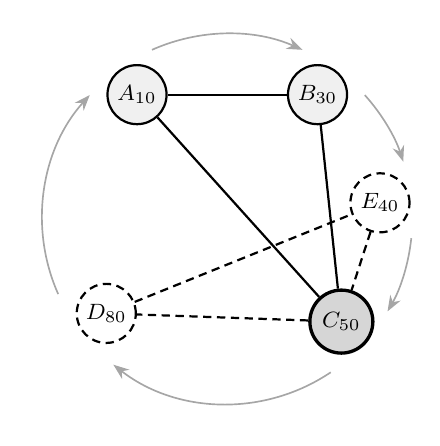
\begin{tikzpicture}[
  node distance=1.4cm,
  peerv1/.style={circle,draw=black,thick,fill=gray!12,minimum size=7.5mm,inner sep=1pt,font=\footnotesize\bfseries},
  peerbridge/.style={circle,draw=black,very thick,fill=gray!32,minimum size=8.0mm,inner sep=1pt,font=\footnotesize\bfseries},
  peerv2/.style={circle,draw=black,thick, densely dashed,fill=white,minimum size=7.5mm,inner sep=1pt,font=\footnotesize\bfseries},
  ringarc/.style={-{Stealth[length=2mm]},semithick,gray!70},
  linkv1/.style={thick},
  linkv2/.style={thick,densely dashed}
]
  \def\R{1.95cm}
  \node[peerv1]     (A) at (126:\R) {$A_{10}$};
  \node[peerv1]     (B) at (54:\R)  {$B_{30}$};
  \node[peerv2]     (E) at (6:\R)   {$E_{40}$};
  \node[peerbridge] (C) at (-42:\R) {$C_{50}$};
  \node[peerv2]     (D) at (-142:\R){$D_{80}$};

  % Physical links in V1 (solid)
  \draw[linkv1] (A) -- (B);
  \draw[linkv1] (B) -- (C);
  \draw[linkv1] (A) -- (C);

  % Physical links in V2 (dashed)
  \draw[linkv2] (C) -- (D);
  \draw[linkv2] (D) -- (E);
  \draw[linkv2] (E) -- (C);

  % Ring orientation outside
  \draw[ringarc] (114:2.35cm) arc (114:66:2.35cm);
  \draw[ringarc] (42:2.35cm)  arc (42:18:2.35cm);
  \draw[ringarc] (-6:2.35cm)  arc (-6:-30:2.35cm);
  \draw[ringarc] (-56:2.35cm) arc (-56:-128:2.35cm);
  \draw[ringarc] (-156:2.35cm) arc (-156:-222:2.35cm);
\end{tikzpicture}
\caption{Interleaved ring $A(10) \to B(30) \to E(40) \to C(50) \to D(80)$ over
two non-transitive WebRTC cliques $V_1 = \{A,B,C\}$ (solid links) and
$V_2 = \{C,D,E\}$ (dashed links) sharing bridge node $C(50)$.}
\label{fig:interleaved-ring}
\end{figure}

Figure~\ref{fig:interleaved-ring} illustrates this configuration. In $V_1$,
the sub-ring successor of $B(30)$ is $C(50)$; in $V_2$, the sub-ring successor
of $E(40)$ is also $C(50)$, while the sub-ring successor of $D(80)$ is $E(40)$.
Tracing standard stabilization and routing over~\eqref{eq:interleaved-order}
exposes three coupled defects:

\subsection{Failure Mode 1: Empty-Confirmed Report Drop and Dial Amplification}
When a node $u$ receives a stabilization report $\texttt{reported}$ from its
current head $r = \Head(u)$, it dials bounded unknown candidates and then
filters the report under the transport lifecycle lock to retain only routable
peers:
\begin{multline*}
  \texttt{confirmed} = \texttt{reported}.\operatorname{confirmed\_by}\\
  \bigl(p \mapsto p = u \lor \operatorname{Routable}(u, p)\bigr).
\end{multline*}
Suppose $r = C(50)$ reports only peers in $V_2 \setminus \{C\} = \{D, E\}$ to a
node $u \in V_1 \setminus \{C\}$ (for instance before $C$ has populated $A$ or
$B$ into its successor list, or when $K$ slots at $C$ are occupied by nodes of
$V_2$). Because $u$ cannot complete ICE with $D$ or $E$, $\texttt{confirmed}$ is
empty ($\neg\texttt{confirmed}.\operatorname{has\_confirmed\_peer}()$). Guarding
the commit on $\texttt{confirmed}.\operatorname{has\_confirmed\_peer}()$ aborts
the stabilization transition entirely: $u$ never commits
$\texttt{Stabilize}(r)$, never emits $\texttt{Notify}(r)$ to inform $C$ of $u$'s
existence, and on the next periodic tick after pending handshake expiry, $u$
re-dials $D$ and $E$ from scratch, generating an unbounded stream of relayed
\texttt{ConnectNodeSend} SDP offers across $C$.

\subsection{Failure Mode 2: Single-Predecessor Preemption at Articulation Nodes}
In~\eqref{eq:interleaved-order}, both $B(30) \in V_1$ and $E(40) \in V_2$ have
$\Head(B) = \Head(E) = C(50)$ within their respective reachable sub-cliques, so
both send $\texttt{Notify}(C)$. Under a single predecessor register
$\texttt{predecessor}: \operatorname{Option}\langle\operatorname{Did}\rangle$,
the update rule
\[
  \operatorname{rectify}(n, p_{\text{cur}}, p_{\text{cand}}) :
  \dist(n, p_{\text{cand}}) > \dist(n, p_{\text{cur}})
\]
retains only $E(40)$ at $C(50)$ because $\dist(C(50), E(40)) = 246 >
\dist(C(50), B(30)) = 236$. Whenever $B(30)$ notifies $C(50)$ first and $E(40)$
notifies second, $E(40)$ overwrites $B(30)$; whenever $E(40)$ notifies first and
$B(30)$ notifies second, $B(30)$ is ignored. Consequently:
\begin{enumerate}
  \item When $C(50)$ answers $B(30)$'s stabilization query, $C(50)$ reports only
  $\texttt{predecessor} = \operatorname{Some}(E(40))$, which $B(30)$ strips as
  unroutable. Thus $B(30)$ observes $\texttt{confirmed.predecessor} =
  \operatorname{None} \neq \operatorname{Some}(B(30))$ and can never prove its
  local finger range $[0..\ell(B, C)]$~\cite{Zave2017}.
  \item If $|V_2 \setminus \{C\}| \ge K$, $C$'s capacity-$K$ successor list is
  filled by nodes of $V_2$, so $B(30)$ is absent from both $C$'s successor list
  and $C$'s single predecessor slot, leaving $B(30) \notin \Referenced(C)$ and
  exposing the critical bridge link $(B, C)$ to connection-capacity eviction.
\end{enumerate}

\subsection{Failure Mode 3: Routing Dead-End and False Local Termination}
Consider a payload originated by $E(40)$ or $D(80)$ in $V_2$ toward $A(10)$ or
$B(30)$ in $V_1$:
\begin{enumerate}
  \item At $E(40)$, the linked known peers are $\{C(50), D(80)\}$. For target
  $A(10)$, $\dist(E(40), A(10)) = 226$, while $\dist(E(40), C(50)) = 10$ and
  $\dist(E(40), D(80)) = 40$. Both $C(50)$ and $D(80)$ lie in the half-open arc
  $(E(40), A(10)]$. Greedy clockwise forwarding selects
  $\arg\max_{p \in (E, A]} \dist(E, p) = D(80)$, sending the packet \emph{away}
  from the bridge $C(50)$ to $D(80)$.
  \item At $D(80)$, the linked known peers are $\{E(40), C(50)\}$ at distances
  $\dist(D(80), E(40)) = 216$ and $\dist(D(80), C(50)) = 226$, both strictly
  greater than $\dist(D(80), A(10)) = 186$. Thus no linked peer of $D(80)$ lies
  in $(D(80), A(10)]$.
  \item Standard single-crossing handoff at $D(80)$ forwards to the nearest
  clockwise linked peer $\arg\min_{p} \dist(D(80), p) = E(40)$ with
  $\texttt{handed\_off} = \top$.
  \item Upon returning to $E(40)$ with $\texttt{handed\_off} = \top$, greedy
  forwarding again selects $D(80)$, where a second crossing is refused and the
  packet is dropped ($\perp$).
\end{enumerate}
Thus the entire trace $E(40) \to D(80) \xrightarrow{\text{handoff}} E(40) \to
D(80) \to \perp$ bypasses bridge $C(50)$ and fails to deliver, even though a
2-hop physical path $E(40) \to C(50) \to A(10)$ (and $D(80) \to C(50) \to
A(10)$) exists in $G$.

\subsection{Why Unstructured Gossip and Virtual Fingers Are Inadmissible}
Two classical workarounds from the peer-to-peer literature are incompatible
with the resource and safety invariants of \texttt{rings-core}:
\begin{itemize}
  \item \textbf{Unstructured 1-hop neighborhood gossip} (broadcasting all active
  connections in \texttt{TopoInfo} and dialing every 2-hop neighbor) inflates
  \texttt{TopoInfo} from $O(K)$ to $O(\operatorname{deg}(n))$ and triggers
  $O(N^2)$ WebRTC SDP offer storms across bridge nodes, violating the $O(1)$
  control-message bound and per-slot memory accounting.
  \item \textbf{Global virtual links in \texttt{FingerTable}}~\cite{Bryan2008,RFC8840}
  (inserting unlinked peers into finger slots and tunneling every Chord hop over
  multi-hop overlays) break the fundamental transport-topology invariant
  $\Referenced(n) \subseteq \Admitted(n)$ and can amplify a single $O(\log N)$
  lookup into $O(\log^2 N)$ physical hops.
\end{itemize}

\section{System Model and State Carrier}

Let $V \subseteq \Ring$ be the set of live nodes and $L \subseteq \binom{V}{2}$
be the set of active, routable WebRTC data-channel links. For each node
$n \in V$, let $\Admitted(n) = \{p \in V \setminus \{n\} : \{n, p\} \in L\}$ be
its set of admitted transport peers, and let $K \ge 1$ denote the successor and
predecessor capacity (\texttt{DEFAULT\_SUCCESSOR\_CAPACITY} $= 3$).

\begin{definition}[Extended Topology Carrier]
The local topology state of node $n \in V$ is the tuple
\begin{multline}
  S_n = \bigl(n,\; \texttt{succ}_n,\; \texttt{pred}_n,\; \texttt{preds}_n,\\
  \texttt{fingers}_n,\; \texttt{bridged}_n,\; \Phi_n,\; \Pi_n\bigr),
\end{multline}
where:
\begin{itemize}
  \item $\texttt{succ}_n \in (V \setminus \{n\})^{\le K}$ is strictly ordered by
  ascending clockwise distance $\dist(n, \cdot)$;
  \item $\texttt{preds}_n \in (V \setminus \{n\})^{\le K}$ is strictly ordered
  by \emph{descending} clockwise distance $\dist(n, \cdot)$ (i.e., ascending
  counter-clockwise distance $\dist(\cdot, n)$);
  \item $\texttt{pred}_n = \texttt{preds}_n.\operatorname{first}() \in
  \operatorname{Option}\langle\operatorname{Did}\rangle$ is the primary
  predecessor projection;
  \item $\texttt{fingers}_n \in (\operatorname{Option}\langle\operatorname{Did}\rangle)^{160}$
  is the sparse/no-wrap direct finger table;
  \item $\texttt{bridged}_n : \operatorname{Did} \rightharpoonup \operatorname{Did}$
  is a finite partial map from unconfirmed remote peer $p$ to an admitted bridge
  reporter $b = \texttt{bridged}_n(p)$;
  \item $\Phi_n$ and $\Pi_n$ are the finger-convergence and pending-stabilization
  protocol states.
\end{itemize}
\end{definition}

\begin{definition}[Referenced Peers and Direct-Link Invariant]
The set of topology-referenced peers at node $n$ is
\begin{multline}
  \Referenced(S_n) = \bigl(\operatorname{set}(\texttt{succ}_n) \cup
  \operatorname{set}(\texttt{preds}_n)\\
  \cup \{p \mid \exists i.\; \texttt{fingers}_n[i] = \operatorname{Some}(p)\}\bigr)
  \setminus \{n\}.
\end{multline}
The state $S_n$ satisfies \texttt{TopologyReferencesOnlyAdmitted} iff
\begin{equation}
  \Referenced(S_n) \subseteq \Admitted(n),
  \label{eq:direct-invariant}
\end{equation}
and every bridge witness satisfies
\begin{multline}
  \forall (p \mapsto b) \in \texttt{bridged}_n:\\
  p \neq n \;\land\; b \in \Referenced(S_n) \;\land\; p \notin \Referenced(S_n).
  \label{eq:bridge-invariant}
\end{multline}
\end{definition}

Equations~\eqref{eq:direct-invariant} and~\eqref{eq:bridge-invariant} preserve a
strict separation of concerns: $\Referenced(S_n)$ contains \emph{only} directly
admitted WebRTC peers (protecting all of $\texttt{succ}_n$, $\texttt{preds}_n$,
and $\texttt{fingers}_n$ from unreferenced-connection eviction), while
$\texttt{bridged}_n$ stores passive 1-hop reachability hints whose `via` peer
$b$ is always an admitted member of $\Referenced(S_n)$.

\section{Bounded Multi-Predecessor Stabilization}

\subsection{Empty-Confirmed Commit and Candidate Dial Backoff}
When node $n$ processes an authenticated stabilization report $\texttt{reported}$
from $r$ echoing the active token $\texttt{request\_id}$, $n$ partitions the
advertised peers under the lifecycle lock using the routability predicate
$\rho_n(p) \equiv (p = n) \lor \operatorname{Routable}(n, p)$:
\begin{align}
  \texttt{confirmed}   &= \texttt{reported}.\operatorname{confirmed\_by}(\rho_n), \\
  \texttt{unconfirmed} &= \texttt{reported}.\operatorname{unconfirmed\_peers}(n, \rho_n).
\end{align}
So long as the reporter itself remains an active routable connection
($\operatorname{Routable}(n, r)$), $n$ commits the stabilization transition even
when $\texttt{confirmed}$ contains no peers:
\begin{multline}
  \operatorname{Routable}(n, r) \implies\\
  \operatorname{commit}\bigl(\texttt{Stabilize}(r, \texttt{request\_id},\\
  \texttt{confirmed}, \texttt{unconfirmed})\bigr).
  \label{eq:empty-confirmed-commit}
\end{multline}
Because $r = \Head(n) \in \texttt{succ}_n$ is already confirmed by
$\operatorname{Routable}(n, r)$, $\Head(\texttt{next\_succ}_n)$ remains
non-empty and emits $\texttt{Notify}(r)$, breaking the notification deadlock of
Failure Mode~1.

To prevent repeated SDP offers toward unreachable candidates across periodic
stabilization ticks, each transport maintains a bounded negative-cache
$\mathcal{B}_n : \operatorname{Did} \rightharpoonup (\text{failures} \in
\mathbb{N}^+, \text{retry\_after\_ms} \in \mathbb{N})$ of capacity $B_{\max} =
64$. Whenever an unadmitted handshake attempt for candidate $c$ fails or expires
before admission, $\mathcal{B}_n$ records a cooldown
\begin{equation}
  \Delta_{\text{backoff}}(f) = \min\bigl(\Delta_0 \cdot 2^{\min(f-1, 4)},\;
  \Delta_{\max}\bigr),
\end{equation}
with $\Delta_0 = 30\,\text{s}$ and $\Delta_{\max} = 300\,\text{s}$. Automatic
DHT candidate dials (\texttt{ConnectDhtPeer}) skip $c$ while
$\text{now\_ms} < \text{retry\_after\_ms}(c)$, whereas explicit application
connects (\texttt{Swarm::connect}) bypass and clear $\mathcal{B}_n(c)$, and
successful admission of $c$ immediately clears $\mathcal{B}_n(c)$.

\subsection{Multi-Predecessor Rectification Law}
Let $\operatorname{can\_rectify}(S_n, c)$ be the geometric admissibility
predicate requiring $c \neq n$ and $c \notin (n, \Head(S_n))$ (with
$c = \Head(S_n)$ allowed only on a two-node wrapping ring). We define the
bounded multi-predecessor rectification operator
$\operatorname{rectify\_preds}(S_n, c, K)$ as follows:
\begin{definition}[Supersede-on-Closer, Retain-on-Sub-Ring]
Given state $S_n$, candidate $c$, and capacity $K \ge 1$:
\begin{enumerate}
  \item If $\neg\operatorname{can\_rectify}(S_n, c)$ or $K = 0$, return
  $\texttt{preds}_n$.
  \item Let $p_0 = \texttt{preds}_n.\operatorname{first}()$.
  \item \textbf{(Supersede on closer joiner)} If $p_0 = \operatorname{None}$ or
  $\dist(n, c) > \dist(n, p_0)$, then $c$ lies strictly between $p_0$ and $n$ on
  $\Ring$; return the singleton $[c]$ (any sub-ring predecessor behind $c$ that
  cannot reach $c$ will re-notify $n$ on its next stabilization tick).
  \item \textbf{(Retain on sub-ring notification)} If $\dist(n, c) \le
  \dist(n, p_0)$, insert $c$ into $\texttt{preds}_n$, sort by descending
  $\dist(n, \cdot)$, deduplicate, and truncate to $K$.
\end{enumerate}
\label{def:rectify-preds}
\end{definition}

\begin{lemma}[Transitive Fixpoint Collapse and Articulation Retention]
\label{lem:articulation-retention}
Under Definition~\ref{def:rectify-preds}:
\begin{enumerate}
  \item On any transitive ring $(V, \binom{V}{2})$ after stabilization
  converges, only the unique global predecessor $p^* = \Pred_V(n)$ has
  $\Head(p^*) = n$; hence $\texttt{preds}_n = [p^*]$ of length $1$.
  \item On a non-transitive graph $G = (V, L)$ where $m \le K$ cliques
  $V_1, \dots, V_m$ meet at articulation node $C$, let $p_i = \Pred_{V_i}(C)$
  be $C$'s predecessor in each clique $V_i$. Because $\Head_{V_i}(p_i) = C$,
  each $p_i$ periodically commits stabilization against $C$ and emits
  $\texttt{Notify}(C)$. Within at most two stabilization rounds after the last
  join, $\texttt{preds}_C$ retains all $m$ predecessors ordered by descending
  $\dist(C, p_i)$, and $\{p_1, \dots, p_m\} \subseteq \Referenced(S_C)$.
\end{enumerate}
\end{lemma}
\begin{proof}
Part~(1) follows because any earlier predecessor $q$ with $\dist(n, q) <
\dist(n, p^*)$ is superseded when $p^*$ notifies $n$, and once $q$ learns $p^*$
from $n$'s \texttt{TopoInfo}, transitivity allows $q$ to connect to $p^*$ and
move its head into $(q, p^*]$, so $q$ never notifies $n$ again. For Part~(2),
let $p_{(1)}, \dots, p_{(m)}$ be ordered so that $\dist(C, p_{(1)}) > \dots >
\dist(C, p_{(m)})$. Once $p_{(1)}$ notifies $C$, $\texttt{preds}_C[0] = p_{(1)}$
can never be superseded by any $p_{(j)}$ ($j > 1$). On the subsequent
stabilization tick of each $p_{(j)}$ ($j > 1$), \eqref{eq:empty-confirmed-commit}
commits $p_{(j)}$'s report from $C$ and emits $\texttt{Notify}(C)$, which
satisfies Clause~4 of Definition~\ref{def:rectify-preds} and inserts $p_{(j)}$
into $\texttt{preds}_C$ up to capacity $K \ge m$. Since
$\operatorname{set}(\texttt{preds}_C) \subseteq \Referenced(S_C)$, connection
eviction never retires any $p_{(j)}$.
\end{proof}

\subsection{Local Finger Range Proof under Multi-Predecessor Reports}
Each \texttt{TopoInfo} frame serialized by reporter $r$ carries both
$\texttt{successors} = \texttt{succ}_r$ and
$\texttt{predecessors} = \texttt{preds}_r$ (at most $2K$ DIDs in total). When
receiver $n$ filters $r$'s report via $\operatorname{confirmed\_by}(\rho_n)$,
\begin{align}
  \texttt{confirmed.preds} &= [p \in \texttt{reported.preds} \mid \rho_n(p)], \\
  \texttt{confirmed.pred}  &= \texttt{confirmed.preds}.\operatorname{first}().
\end{align}

\begin{lemma}[Sub-Clique Local Finger Proof]
\label{lem:subclique-proof}
In the two-clique ring~\eqref{eq:interleaved-order}, once $C(50)$ holds
$\texttt{preds}_C = [E(40), B(30)]$, $B(30)$'s confirmation filter over $C$'s
report yields $\texttt{confirmed.preds} = [B(30)]$ and
$\texttt{confirmed.pred} = \operatorname{Some}(B(30))$. Consequently,
\texttt{stabilized\_successor\_proof\_end} at $B(30)$ proves all finger slots
$i$ with $2^i \le \dist(B(30), C(50))$ to $C(50)$.
\end{lemma}
\begin{proof}
At $B(30)$, $\rho_B(E(40)) = \bot$ and $\rho_B(B(30)) = \top$. Thus the closest
routable predecessor of $C(50)$ in $B(30)$'s clique $V_1$ is $B(30)$ itself, so
$\texttt{confirmed.pred} = \operatorname{Some}(B(30))$. Since $\Head(S_B) =
\Head(\texttt{next\_succ}_B) = C(50)$ and no peer in $\Admitted(B)$ lies in
$(B(30), C(50))$, $C(50)$ is the exact direct finger for every slot threshold
$2^i \le \dist(B(30), C(50))$.
\end{proof}

\section{Passive Gap-Bridge Hints and Owner Lookup}

\subsection{Zero-TTL Passive Hint Lifecycle}
Whenever node $n$ processes an authenticated \texttt{TopoInfo} report from an
admitted successor $r \in \texttt{succ}_n$ (via either
\texttt{QueryFor::Stabilization} or \texttt{QueryFor::SyncSuccessor}), the
unconfirmed peers
\begin{multline*}
  U(n, r) = \bigl(\operatorname{set}(\texttt{reported.preds}) \\
  \cup \operatorname{set}(\texttt{reported.succ})\bigr) \setminus
  \{p \mid \rho_n(p)\}
\end{multline*}
are peers to which $r$ holds an active link ($\{r, p\} \in L$) while $n$ does
not ($\{n, p\} \notin L$). The pure transition updates $\texttt{bridged}_n$
according to three deterministic rules:
\begin{enumerate}
  \item \textbf{Report refresh (\texttt{Stabilize} / \texttt{SyncSuccessor}):}
  Remove all prior entries $(p \mapsto b) \in \texttt{bridged}_n$ with $b = r$,
  then for each $p \in U(n, r)$ with $p \notin \Referenced(S'_n)$, insert
  $p \mapsto r$.
  \item \textbf{Direct admission (\texttt{Admit}$(p)$):} Remove $p$ from
  $\operatorname{dom}(\texttt{bridged}_n)$ because $p$ is now directly linked.
  \item \textbf{Peer removal (\texttt{Remove}$(p)$):} Retain only entries
  $(t \mapsto b) \in \texttt{bridged}_n$ with $t \neq p \land b \neq p$.
\end{enumerate}

\begin{lemma}[Boundedness and Liveness of $\texttt{bridged}_n$]
For every reachable state $S_n$, $|\texttt{bridged}_n| \le 2K \cdot |\texttt{succ}_n|
\le 2K^2$, and every entry $(p \mapsto b) \in \texttt{bridged}_n$ is backed by a
currently referenced successor $b \in \Referenced(S_n)$ and refreshed on every
stabilization or successor-sync round with $b$ without wall-clock TTL timers.
\end{lemma}

\subsection{Gap-Aware \texttt{find\_successor} Preserving \texttt{RoutesClockwise}}
A critical invariant of \texttt{rings-core} (\texttt{invariants.rs}) is
\texttt{RoutesClockwise}:
\begin{multline}
  \operatorname{find\_successor}(S_n, \mathit{id}) =
  \operatorname{Remote}(\mathit{next}, \mathit{id}) \\
  \implies \mathit{next} \in (n, \mathit{id}),
  \label{eq:routes-clockwise}
\end{multline}
i.e., $0 < \dist(n, \mathit{next}) < \dist(n, \mathit{id})$. Forwarding to
$\Head(S_n)$ when $\dist(n, \mathit{id}) < \dist(n, \Head(S_n))$ would violate
\eqref{eq:routes-clockwise}. However, when $\mathit{id} \in (n, \Head(S_n)]$
($\mathit{id} \neq n$), any peer $p \in (n, \Head(S_n))$ advertised by the
bridge is \emph{already present} in $\operatorname{dom}(\texttt{bridged}_n)$!
Furthermore, any direct predecessor $p \in \texttt{preds}_n$ is a known live
member of the ring. We therefore define gap-aware \texttt{find\_successor} as:
\begin{enumerate}
  \item If $\mathit{id} \neq n$ and $\mathit{id} \in \texttt{preds}_n$, return
  $\operatorname{Local}(\mathit{id})$.
  \item Let $h = \Head(S_n)$ and $t = \dist(n, \mathit{id})$. If $t \le \dist(n, h)$:
  \begin{itemize}
    \item If $\mathit{id} = n$, return $\operatorname{Local}(h)$.
    \item Let $B_{\text{gap}} = \{p \in \operatorname{dom}(\texttt{bridged}_n) \mid
    \texttt{bridged}_n(p) \in \Referenced(S_n) \;\land\;
    t \le \dist(n, p) < \dist(n, h)\}$.
    \item If $B_{\text{gap}} \neq \emptyset$, return
    $\operatorname{Local}\bigl(\arg\min_{p \in B_{\text{gap}}} \dist(n, p)\bigr)$;
    otherwise return $\operatorname{Local}(h)$.
  \end{itemize}
  \item If $t > \dist(n, h)$, select $\mathit{next} = \arg\max\{\dist(n, p) \mid
  p \in \Referenced(S_n) \setminus \{n\},\; \dist(n, p) < t\}$ (scanning
  $\texttt{fingers}_n$, $\texttt{succ}_n$, and $\texttt{preds}_n$), returning
  $\operatorname{Remote}(\mathit{next}, \mathit{id})$ if such a $p$ exists and
  $\operatorname{Local}(h)$ otherwise.
\end{enumerate}

\begin{lemma}[Preservation of \texttt{RoutesClockwise}]
Gap-aware \texttt{find\_successor} satisfies~\eqref{eq:routes-clockwise} for
every representable state $S_n$ and every target $\mathit{id} \in \Ring$.
\end{lemma}
\begin{proof}
Clauses~1 and~2 return $\operatorname{Local}(\cdot)$, which satisfies
\eqref{eq:routes-clockwise} vacuously. Clause~3 emits
$\operatorname{Remote}(\mathit{next}, \mathit{id})$ only for candidates
satisfying $\mathit{next} \neq n$ and $\dist(n, \mathit{next}) < t =
\dist(n, \mathit{id})$.
\end{proof}

\section{Bridge-Delegated Delivery and Route Laws}

Payload delivery in \texttt{rings-core} (\texttt{dht::delivery}) tags each frame
with a stage $\sigma = (\texttt{via}, \texttt{handed\_off}) \in
\operatorname{Option}\langle\operatorname{Did}\rangle \times \mathbb{B}$, where
$\Aim(\sigma, T) = \texttt{via}.\operatorname{unwrap\_or}(T)$. We extend
$\operatorname{delivery\_step}(S_n, T, \sigma, \Linked_n)$ with two passive
bridge rules while keeping the wire format of $\RouteStage$ unchanged:
\begin{enumerate}
  \item \textbf{Direct destination links:} If $\Linked_n(T)$, return
  $\operatorname{Some}\bigl((T, \sigma)\bigr)$.
  \item \textbf{Rule B1 (1-Hop Bridge Target Delegation):} If
  $\sigma.\texttt{via} = \operatorname{None}$ and $\texttt{bridged}_n(T) =
  \operatorname{Some}(b)$ with $b \neq n \land \Linked_n(b)$, return
  \begin{equation}
    \operatorname{Some}\Bigl(\bigl(b,\;
    (\operatorname{Some}(b), \sigma.\texttt{handed\_off})\bigr)\Bigr).
    \label{eq:rule-b1}
  \end{equation}
  \item \textbf{Explicit aim resolution:} Let $a = \Aim(\sigma, T)$. If $a \neq T$:
  if $a = n$ return $\operatorname{None}$ (the bridge lost its link to $T$); if
  $\Linked_n(a)$ return $\operatorname{Some}\bigl((a, \sigma)\bigr)$.
  \item \textbf{Rule B2 (Gap-Bridge Handoff):} Evaluate
  $\operatorname{route\_toward}(S_n, a, \Linked_n)$ over
  $\Known(S_n) \cap \Linked_n$, where $\Known(S_n) = \Referenced(S_n)$.
  \begin{itemize}
    \item On $\operatorname{Forward}(p)$, return $\operatorname{Some}\bigl((p, \sigma)\bigr)$.
    \item On $\operatorname{Handoff}(h)$ when $\neg\sigma.\texttt{handed\_off}$:
    if $\sigma.\texttt{via} = \operatorname{None}$ and there exists
    $(p \mapsto b) \in \texttt{bridged}_n$ such that $b \neq n$, $\Linked_n(b)$,
    and $\dist(n, p) < \dist(n, h)$ (i.e., $b$ bridges into the local gap
    $(n, h)$ in which $a$ fell), select $b^* = b$ (minimizing $\dist(n, p)$) and
    return $\operatorname{Some}\bigl((b^*, (\operatorname{None}, \top))\bigr)$;
    otherwise return $\operatorname{Some}\bigl((h, (\sigma.\texttt{via}, \top))\bigr)$.
    \item Otherwise return $\operatorname{None}$.
  \end{itemize}
\end{enumerate}

\begin{theorem}[Preservation of Route Safety Laws]
\label{theorem:route-safety}
For any graph $G = (V, L)$, any collection of local views $\{S_n\}_{n \in V}$,
any origin $n_0 \in V$, destination $T \in V$, and initial stage $\sigma_0$, the
sequence of states $(n_0, \sigma_0), (n_1, \sigma_1), \dots$ produced by
$\operatorname{delivery\_step}$ satisfies:
\begin{enumerate}
  \item \textbf{Linked:} Every hop $(n_k, n_{k+1})$ satisfies $\{n_k, n_{k+1}\} \in L$.
  \item \textbf{NeverOvershoots:} For every hop with $n_{k+1} \neq T$,
  $n_{k+1} \neq \Aim(\sigma_{k+1}, T)$, and
  $\neg(\sigma_{k+1}.\texttt{handed\_off} \land \neg\sigma_k.\texttt{handed\_off})$,
  $\dist(n_k, n_{k+1}) < \dist(n_k, \Aim(\sigma_{k+1}, T))$.
  \item \textbf{Acyclic and Bounded:} No state $(n_k, \sigma_k)$ with $n_k \neq T$
  is visited twice, and the total number of hops is at most $2|V|$.
  \item \textbf{Exact Local Delivery:} If $\sigma_0.\texttt{via} = \operatorname{None}$
  and the route terminates undelivered, no visited node $n_k$ had $\{n_k, T\} \in L$.
\end{enumerate}
\end{theorem}
\begin{proof}
(1) Every branch returning $\operatorname{Some}((p, \cdot))$ checks $\Linked_{n_k}(p)$
directly.
(2) Under Rule~B1~\eqref{eq:rule-b1}, $n_{k+1} = b = \Aim(\sigma_{k+1}, T)$, so
the precondition $n_{k+1} \neq \Aim(\sigma_{k+1}, T)$ is false. Under Rule~B2,
$\sigma_k.\texttt{handed\_off} = \bot$ and $\sigma_{k+1}.\texttt{handed\_off} =
\top$, so the crossing guard holds. Under $\operatorname{Forward}(p)$,
$p \in (n_k, a]$ with $p \neq a \implies \dist(n_k, p) < \dist(n_k, a)$.
(3) Within each fixed stage $\sigma$, $\dist(n_k, \Aim(\sigma, T))$ strictly
decreases in $\mathbb{N}$ on every $\operatorname{Forward}$ step, visiting at
most $|V|-1$ nodes. The boolean $\texttt{handed\_off}$ transitions $\bot \to
\top$ at most once. Rule~B1 transitions $\texttt{via}$ from $\operatorname{None}$
to $\operatorname{Some}(b)$ and jumps directly to $n_{k+1} = b$; at $b$, either
$\Linked_b(T)$ delivers in one final hop ($n_{k+2} = T$) or $a = b = \text{local}$
terminates immediately with $\operatorname{None}$. Hence Rule~B1 cannot
introduce any cycle and adds at most one intermediate node $b$ (which was not the
destination). Thus the route visits at most $2|V|$ hops.
(4) Clause~1 checks $\Linked_{n_k}(T)$ before any other rule, so no node linked
to $T$ can fail to deliver to $T$.
\end{proof}

\begin{theorem}[All-Pairs Delivery Across Bridge-Connected Cliques]
\label{theorem:all-pairs}
Let $G = (V, L)$ consist of two cliques $V_1, V_2$ sharing bridge node $C$ with
$|V_1 \setminus \{C\}| \le K$ and $|V_2 \setminus \{C\}| \le K$. Once each node
in $V_1 \cup V_2$ has processed one stabilization report from its sub-clique
head and (for nodes whose non-head successor is $C$) one successor-sync report
from $C$, every ordered pair $(u, v) \in V \times V$ ($u \neq v$) delivers in at
most $2$ hops (and in at most $3$ hops even before non-head successor sync with
$C$ completes).
\end{theorem}
\begin{proof}
If $u$ and $v$ belong to the same clique $V_i$, then $\{u, v\} \in L$ and
Clause~1 delivers in $1$ hop ($u \to v$). Otherwise, suppose $u \in V_i \setminus
\{C\}$ and $v \in V_j \setminus \{C\}$ ($i \neq j$). By
Lemma~\ref{lem:articulation-retention}, $\Referenced(S_C) = (V_1 \cup V_2)
\setminus \{C\}$, and every peer $v \in V_j \setminus \{C\}$ appears in $C$'s
\texttt{TopoInfo} ($\texttt{succ}_C \cup \texttt{preds}_C$). After $u$ receives
$C$'s \texttt{TopoInfo} (via stabilization if $\Head(u) = C$, or via successor
sync since $C \in \texttt{succ}_u$ when $|V_i \setminus \{C\}| \le K$),
$\texttt{bridged}_u(v) = \operatorname{Some}(C)$. Since $\{u, C\} \in L$ and
$\{C, v\} \in L$, Rule~B1 at $u$ forwards to $C$ with stage
$(\operatorname{Some}(C), \bot)$, and Clause~1 at $C$ delivers to $v$, yielding
the 2-hop path $u \to C \to v$. Even before a non-head node $u \in V_i$
completes successor sync with $C$, one greedy or handoff hop inside $V_i$
reaches the sub-clique predecessor $p_i = \Pred_{V_i}(C)$ whose head is $C$;
$p_i$ holds $\texttt{bridged}_{p_i}(v) = \operatorname{Some}(C)$ from
stabilization and applies Rule~B1 to deliver via $p_i \to C \to v$ in $3$ hops.
\end{proof}

\section{Implementation and Verification Summary}

Table~\ref{tab:verification} summarizes the mechanized obligations mapping each
protocol law to the test suites in \texttt{crates/core}.

\begin{table}[t]
\centering
\caption{Mechanized Verification Obligations in \texttt{rings-core}}
\label{tab:verification}
\footnotesize
\begin{tabular}{@{}lll@{}}
\toprule
\textbf{Obligation / Law} & \textbf{Module} & \textbf{Coverage} \\
\midrule
\eqref{eq:empty-confirmed-commit} Empty-confirmed commit & \texttt{transport} & Unit + int. \\
Candidate dial backoff $\mathcal{B}_n$ & \texttt{transport} & Unit test \\
Def.~\ref{def:rectify-preds} Multi-predecessor & \texttt{topology} & Unit + prop. \\
Lemma~\ref{lem:articulation-retention} Retention & \texttt{topology} & Unit test \\
Lemma~\ref{lem:subclique-proof} Sub-clique proof & \texttt{topology} & Unit test \\
Zero-TTL \texttt{bridged} lifecycle & \texttt{topology} & Unit test \\
\eqref{eq:routes-clockwise} \texttt{RoutesClockwise} & \texttt{topology} & Property test \\
Theorem~\ref{theorem:route-safety} Route safety & \texttt{delivery} & Exhaustive \\
Theorem~\ref{theorem:all-pairs} Two-clique delivery & \texttt{delivery} & Model test \\
Stage 6 rejoin BFS invariants & \texttt{rejoin\_model} & 6 BFS models \\
\bottomrule
\end{tabular}
\end{table}

\bibliographystyle{IEEEtran}
\bibliography{non-transitive-chord}

\end{document}
